% Created 2017-09-22 Fri 11:38
\documentclass{ximera}
\newcommand{\RR}{\mathbb R}
\renewcommand{\d}{\,d}
\newcommand{\dd}[2][]{\frac{d #1}{d #2}}
\renewcommand{\l}{\ell}
\newcommand{\ddx}{\frac{d}{dx}}
\newcommand{\dfn}{\textbf}
\newcommand{\eval}[1]{\bigg[ #1 \bigg]}

\author{Jim Fowler and Bart Snapp}
\title{Parameterized curve}

\begin{document}

\begin{abstract}
Explore families of parameterized curves.
\end{abstract}

In what follows, $a$ and $b$ are positive constants.
  
Consider the function $\vec{f} : \R \to \R^2$ given by
\[
  \vec{f}(t) = \vector{ a \cos t, b \sin t }.
\]

\begin{exercise}
  When $a = 2$ and $b = 1$, is it the case that $\vec{f}$ is
  parameterized by arc length?
  \begin{multipleChoice}
    \choice{Yes.}
    \choice[correct]{No.}
  \end{multipleChoice}  
\end{exercise}

\begin{exercise}
  When $a = 1$ and $b = 1$, is it the case that $\vec{f}$ is
  parameterized by arc length?
  \begin{multipleChoice}
    \choice[correct]{Yes.}
    \choice{No.}
  \end{multipleChoice}  
\end{exercise}

\begin{exercise}
  When $a = 2$ and $b = 2$, is it the case that $\vec{f}$ is
  parameterized by arc length?
  \begin{multipleChoice}
    \choice{Yes.}
    \choice[correct]{No.}
  \end{multipleChoice}
\end{exercise}

\begin{exercise}
  Consider this curve:
  \begin{image}
    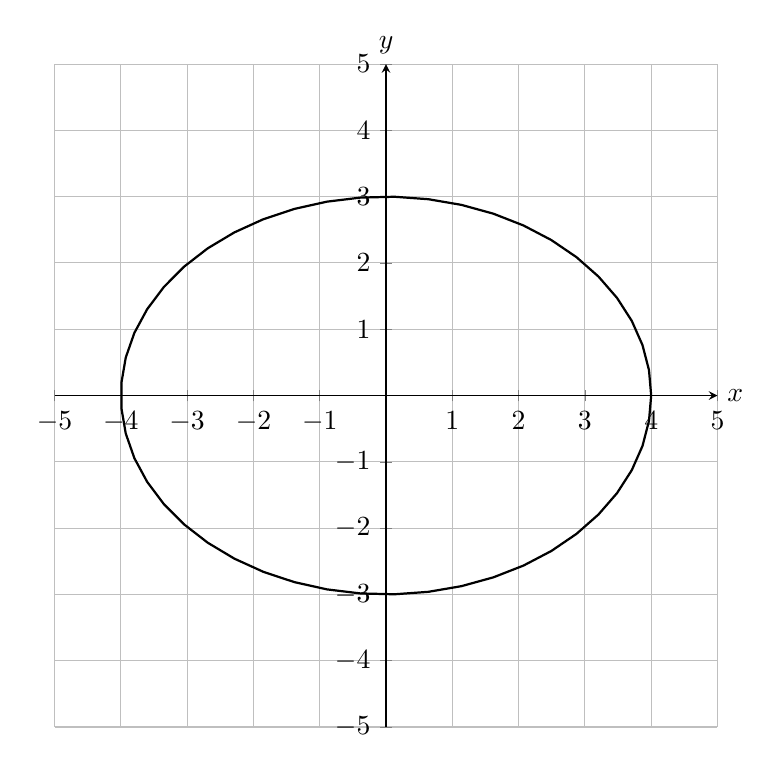
\begin{tikzpicture}
      \begin{axis}[
        xmin=-5,xmax=5,ymin=-5,ymax=5,
        clip=false,
        axis lines=center,
        width=10cm,
        height=10cm,
        xtick={-5,-4,...,5},
        ytick={-5,-4,...,5},
        xlabel=$x$, ylabel=$y$,
        grid = major,
        every axis y label/.style={at=(current axis.above origin),anchor=south},
        every axis x label/.style={at=(current axis.right of origin),anchor=west},
        ]
        \addplot [domain=0:2*pi,samples=50,thick]({4*cos(deg(x))},{3*sin(deg(x))});

      \end{axis}
    \end{tikzpicture}
  \end{image}
  This curve is the image of $\vec{f}(t) = \vector{ a \cos t, b \sin t }$ when $a = \answer{4}$ and $b = \answer{3}$.
\end{exercise}

\begin{exercise}
  Suppose $a = 2$ and $b = 2$, so that $\vec{f}(t) = \vector{ 2 \cos t, 2 \sin t }$.

  Then $\vec{f}'(t) = \vector{\answer{-2 \sin t}, \answer{2 \cos t}}$.
  
  Is $\vec{f}'(t)$ the unit tangent vector to $\vec{f}(t)$?
  \begin{multipleChoice}
    \choice{Yes.}
    \choice[correct]{No.}
  \end{multipleChoice}

  \begin{exercise}
    What is the unit tangent vector to the image of $\vec{f}$ at the point $(\cos t, \sin t)$?
    \[
      \frac{\vec{f}'(t)}{|\vec{f}'(t)|} = \vector{ \answer{ -\sin t } , \answer{ \cos t } }.
    \]
  \end{exercise}
\end{exercise}

\end{document}
